\documentclass{article}

\usepackage{amsmath,graphicx}
\usepackage{sectsty}
\usepackage[letterpaper, margin=0.5cm]{geometry}
\usepackage{amsmath,graphicx}
\usepackage{multicol}
\usepackage{array}
\usepackage{csvsimple}
\usepackage{booktabs}
\usepackage{multirow}
\usepackage{float}
\usepackage{array}

\setlength{\heavyrulewidth}{1.5pt}
\setlength{\abovetopsep}{4pt}

\newcommand{\centered}[1]{\begin{tabular}{l} #1 \end{tabular}}

\graphicspath{./}

\begin{document}
    \begin{center}
        \begin{table}[!htbp]
            \centering
            \caption{Tour Distance Over Time at Various Iteration Counts}
            \begin{tabular}{cccccc}
                \toprule
                \multicolumn{1}{c|}{
                    \parbox[t]{1.5cm}{Number\\ of cities}} & 
                \multicolumn{5}{c}{Number of Iterations} \\
                \midrule
                
                & 50 & 100 & 250 & 500 & 1000 \\
                
                15 &
                \centered{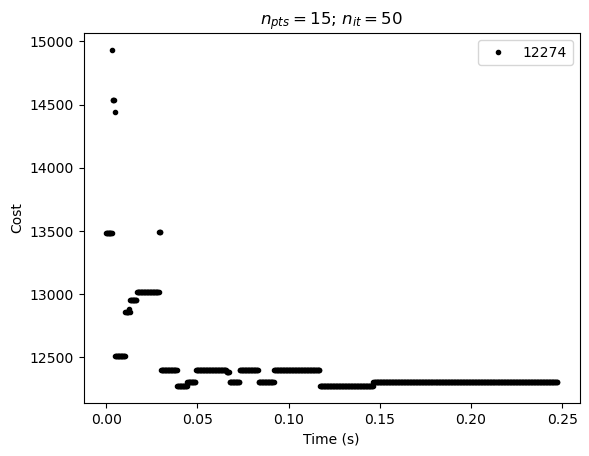
\includegraphics[width=0.14\textwidth]{sVal100/Annealing_15Pts_50it.png}} &
                \centered{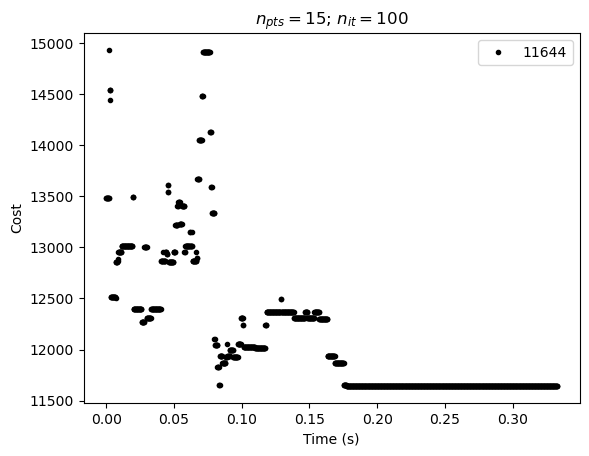
\includegraphics[width=0.14\textwidth]{sVal100/Annealing_15Pts_100it.png}} &
                \centered{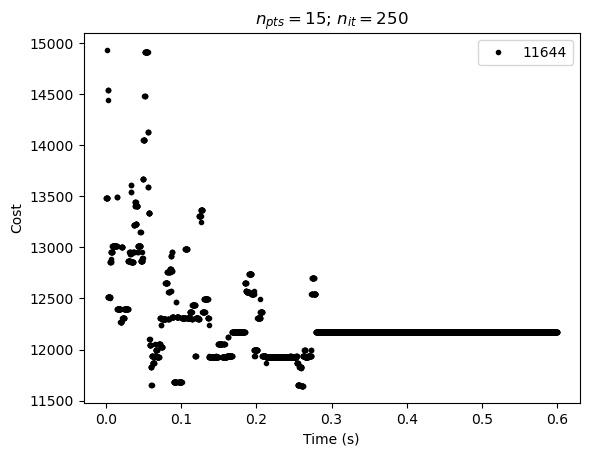
\includegraphics[width=0.14\textwidth]{sVal100/Annealing_15Pts_250it.png}} &
                \centered{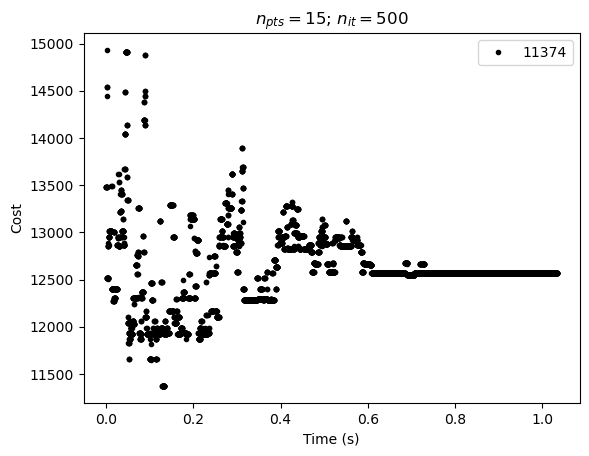
\includegraphics[width=0.14\textwidth]{sVal100/Annealing_15Pts_500it.png}} &
                \centered{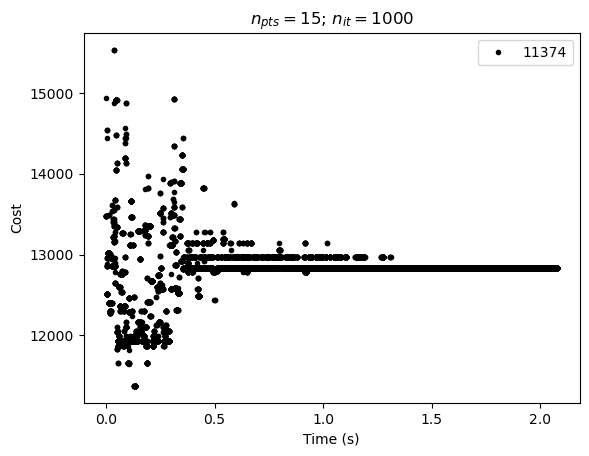
\includegraphics[width=0.14\textwidth]{sVal100/Annealing_15Pts_1000it.png}} \\
                
                30 &
                \centered{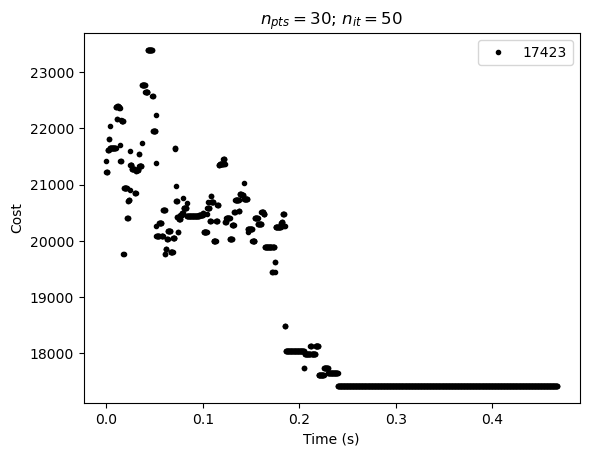
\includegraphics[width=0.14\textwidth]{sVal100/Annealing_30Pts_50it.png}} &
                \centered{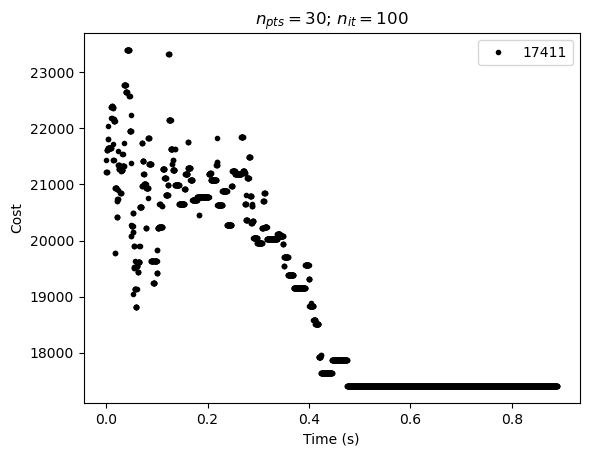
\includegraphics[width=0.14\textwidth]{sVal100/Annealing_30Pts_100it.png}} & 
                \centered{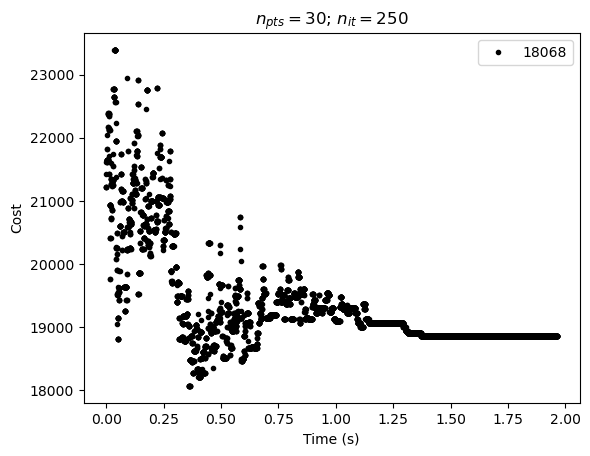
\includegraphics[width=0.14\textwidth]{sVal100/Annealing_30Pts_250it.png}} & 
                \centered{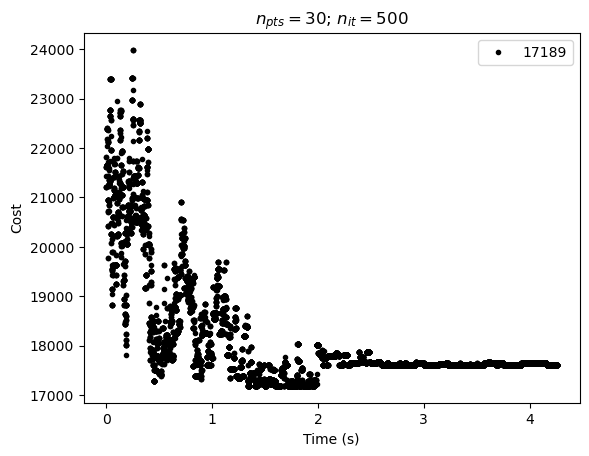
\includegraphics[width=0.14\textwidth]{sVal100/Annealing_30Pts_500it.png}} & 
                \centered{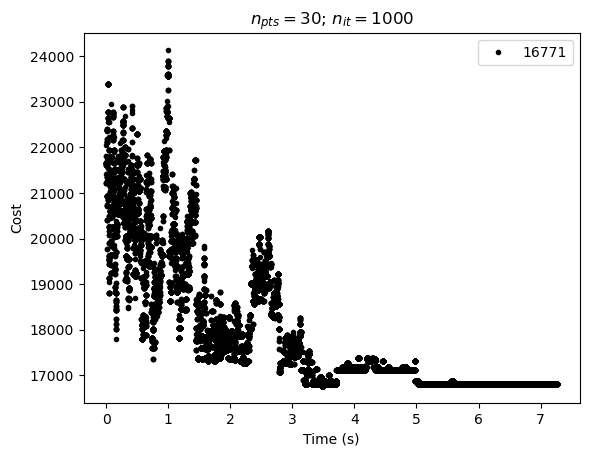
\includegraphics[width=0.14\textwidth]{sVal100/Annealing_30Pts_1000it.png}} \\
                60 &
                \centered{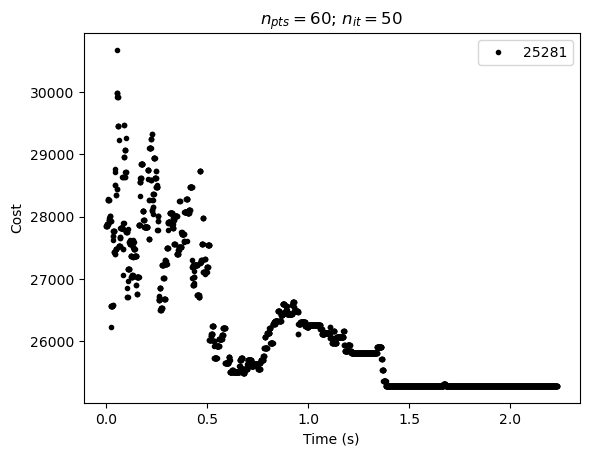
\includegraphics[width=0.14\textwidth]{sVal100/Annealing_60Pts_50it.png}} &
                \centered{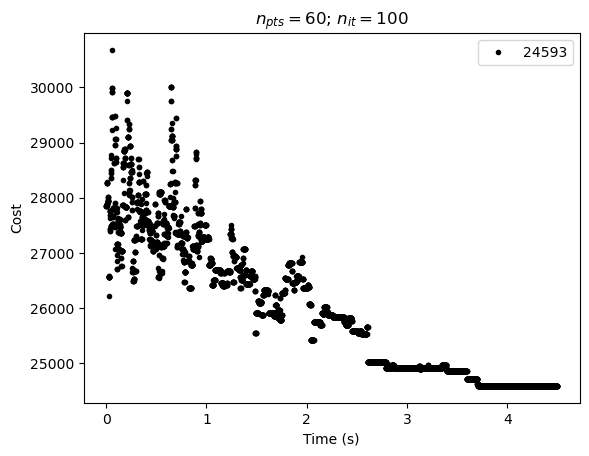
\includegraphics[width=0.14\textwidth]{sVal100/Annealing_60Pts_100it.png}} &
                \centered{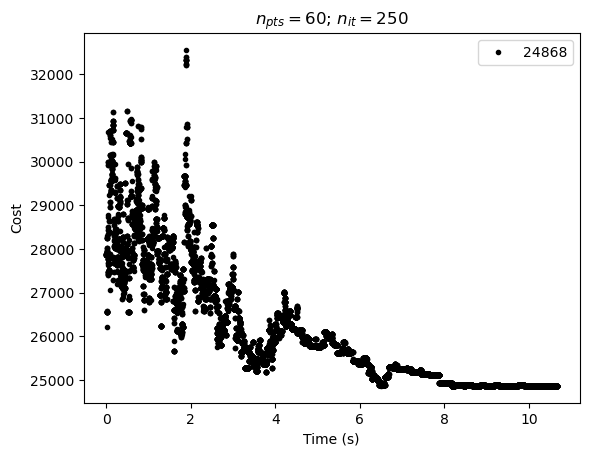
\includegraphics[width=0.14\textwidth]{sVal100/Annealing_60Pts_250it.png}} & 
                \centered{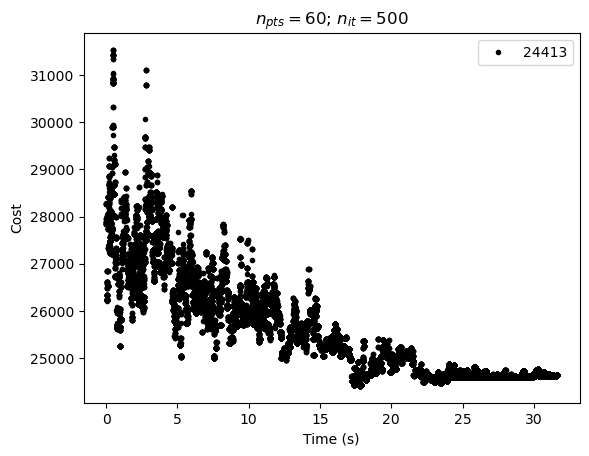
\includegraphics[width=0.14\textwidth]{sVal100/Annealing_60Pts_500it.png}} &
                \centered{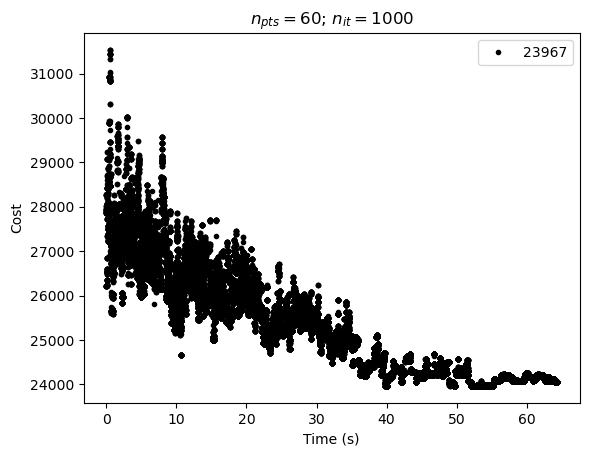
\includegraphics[width=0.14\textwidth]{sVal100/Annealing_60Pts_1000it.png}} \\
                100 &
                \centered{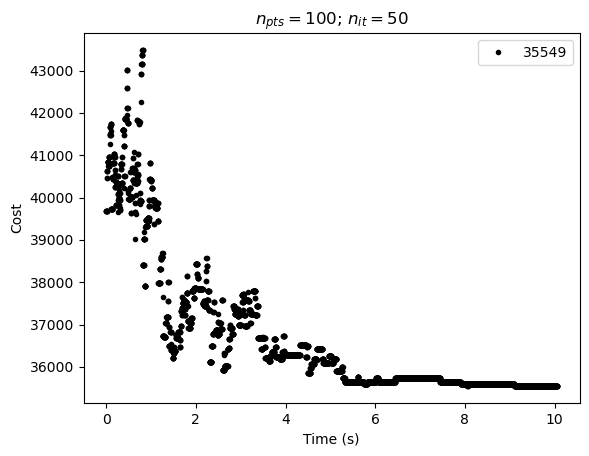
\includegraphics[width=0.14\textwidth]{sVal100/Annealing_100Pts_50it.png}} &
                \centered{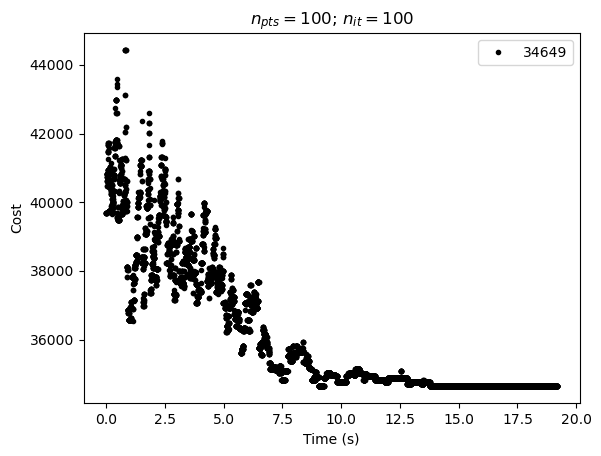
\includegraphics[width=0.14\textwidth]{sVal100/Annealing_100Pts_100it.png}} &
                \centered{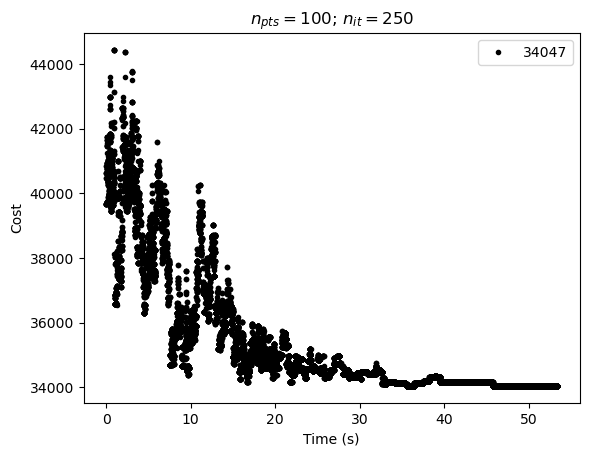
\includegraphics[width=0.14\textwidth]{sVal100/Annealing_100Pts_250it.png}} &
                \centered{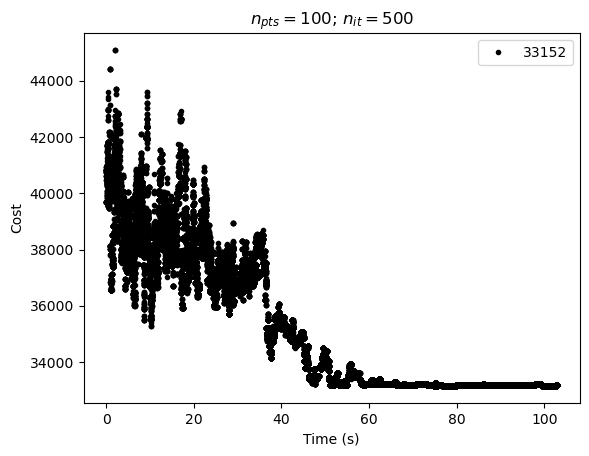
\includegraphics[width=0.14\textwidth]{sVal100/Annealing_100Pts_500it.png}} \\
                %\centered{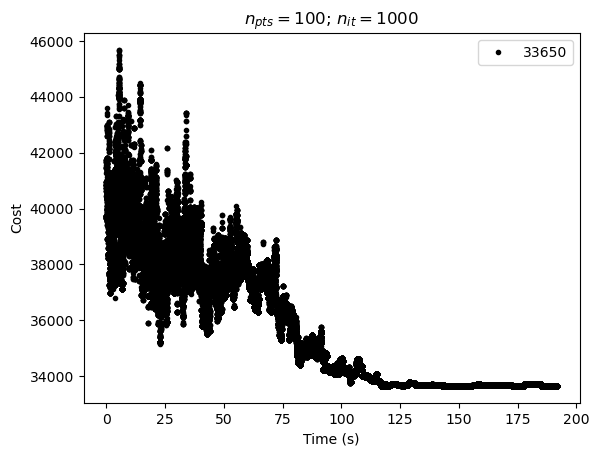
\includegraphics[width=0.14\textwidth]{sVal100/Annealing_100Pts_1000it.png}} &
                200 &
                \centered{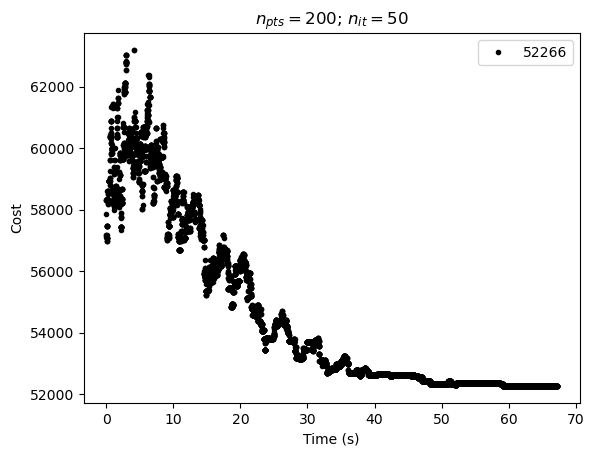
\includegraphics[width=0.14\textwidth]{sVal100/Annealing_200Pts_50it.png}} &
                \centered{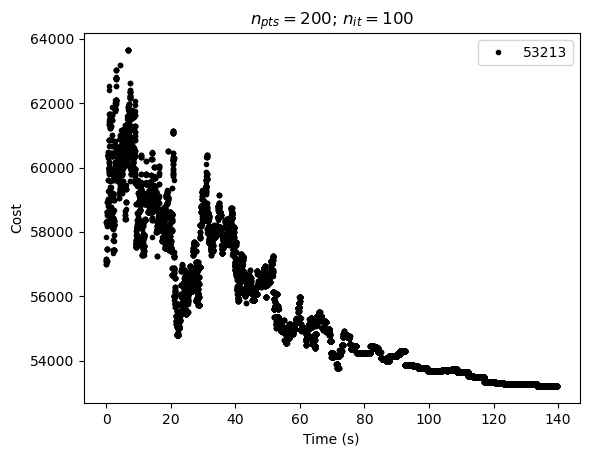
\includegraphics[width=0.14\textwidth]{sVal100/Annealing_200Pts_100it.png}} &
                \centered{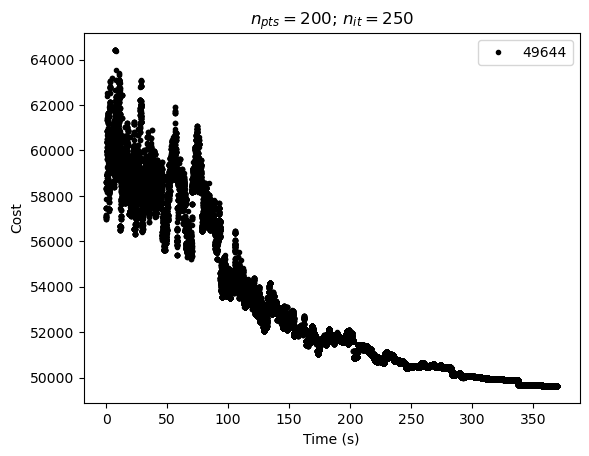
\includegraphics[width=0.14\textwidth]{sVal100/Annealing_200Pts_250it.png}} & 
                \centered{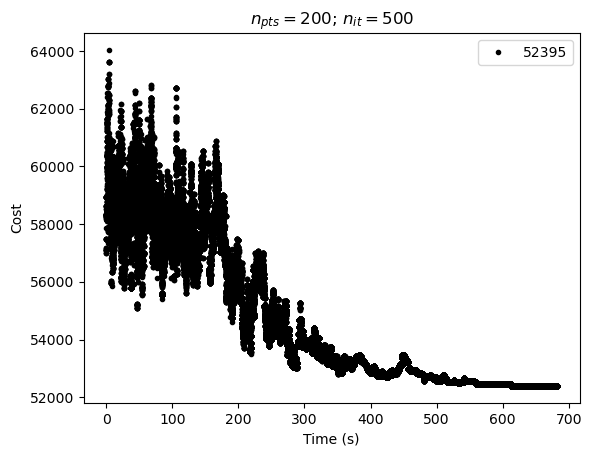
\includegraphics[width=0.14\textwidth]{sVal100/Annealing_200Pts_500it.png}} & 
                \centered{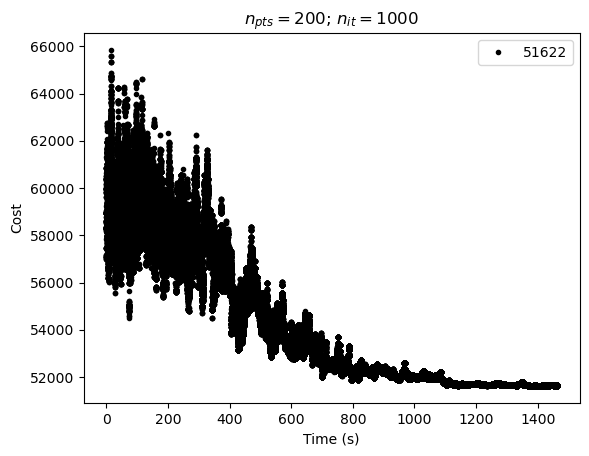
\includegraphics[width=0.14\textwidth]{sVal100/Annealing_200Pts_1000it.png}} \\
            \end{tabular}
        \end{table}

        \begin{tabular}{|c||c|c|c|c|c|}
            \hline
            & 1000 & 500 & 200 & 100 & 50 \\
            \hline\hline
            15 & 25.6\% & 1.0\% & 19.0\% & 3.9 \% & 15.2\% \\
            \hline
            30 & 19.5\% & 18.1\% & 17.6\% & 16.4 \% & 17.5\% \\
            \hline
            60 & 12.8\% & 18.7\% & 18.1\% & 12.6 \% & 15.1\% \\
            \hline
            100 & 16.0\% & 11.8\% & 7.8\% & 11.9 \% & 11.5\% \\
            \hline
            200 & TB & TB & 10.2\% & 13.6\% & 16.3\% \\
            \hline
        \end{tabular}

    \end{center}
    \begin{center}
    \scalebox{0.65}{
        \csvreader[%
        respect all,%
        autotabular%
      ]{data.csv}{}{\csvlinetotablerow}%
    }
    \end{center}

\end{document}
